% vim: tw=80

\chapter{Conclusion}

For the first time, a measurement of triple-differential dijet cross sections
has been achieved at the LHC. 

The measurement was specifically designed in a way to provide constraints on the
PDFs in a best possible way. Up to now, the PDF uncertainties of the PDFs at
high fractional momenta $x$ are sizable, especially the uncertainties of the gluon PDF. 
Because of the omnipresence of the PDFs at the LHC, many analyses would profit
from improvements of the PDFs. In particular searches for new physics at high
energies, in which the highest fractional momenta of the proton are probed,
would benefit from reduced PDF uncertainties.

These challenges were met with the development of a triple-differential dijet
analysis, in which the PDFs are probed over a wide range of $x$ and up to high
transverse momenta. Thus, the cross sections were measured
differentially in the average transverse momentum of the dijet system, \ptavg,
the boost of the dijet system, \yboost, and the rapidity separation of the
two jets, \ystar. It has been shown, that these variables offer a high sensitivity to
the PDFs, especially in the region containing boosted dijet events.

\begin{figure}[h!tbp]
    \centering
    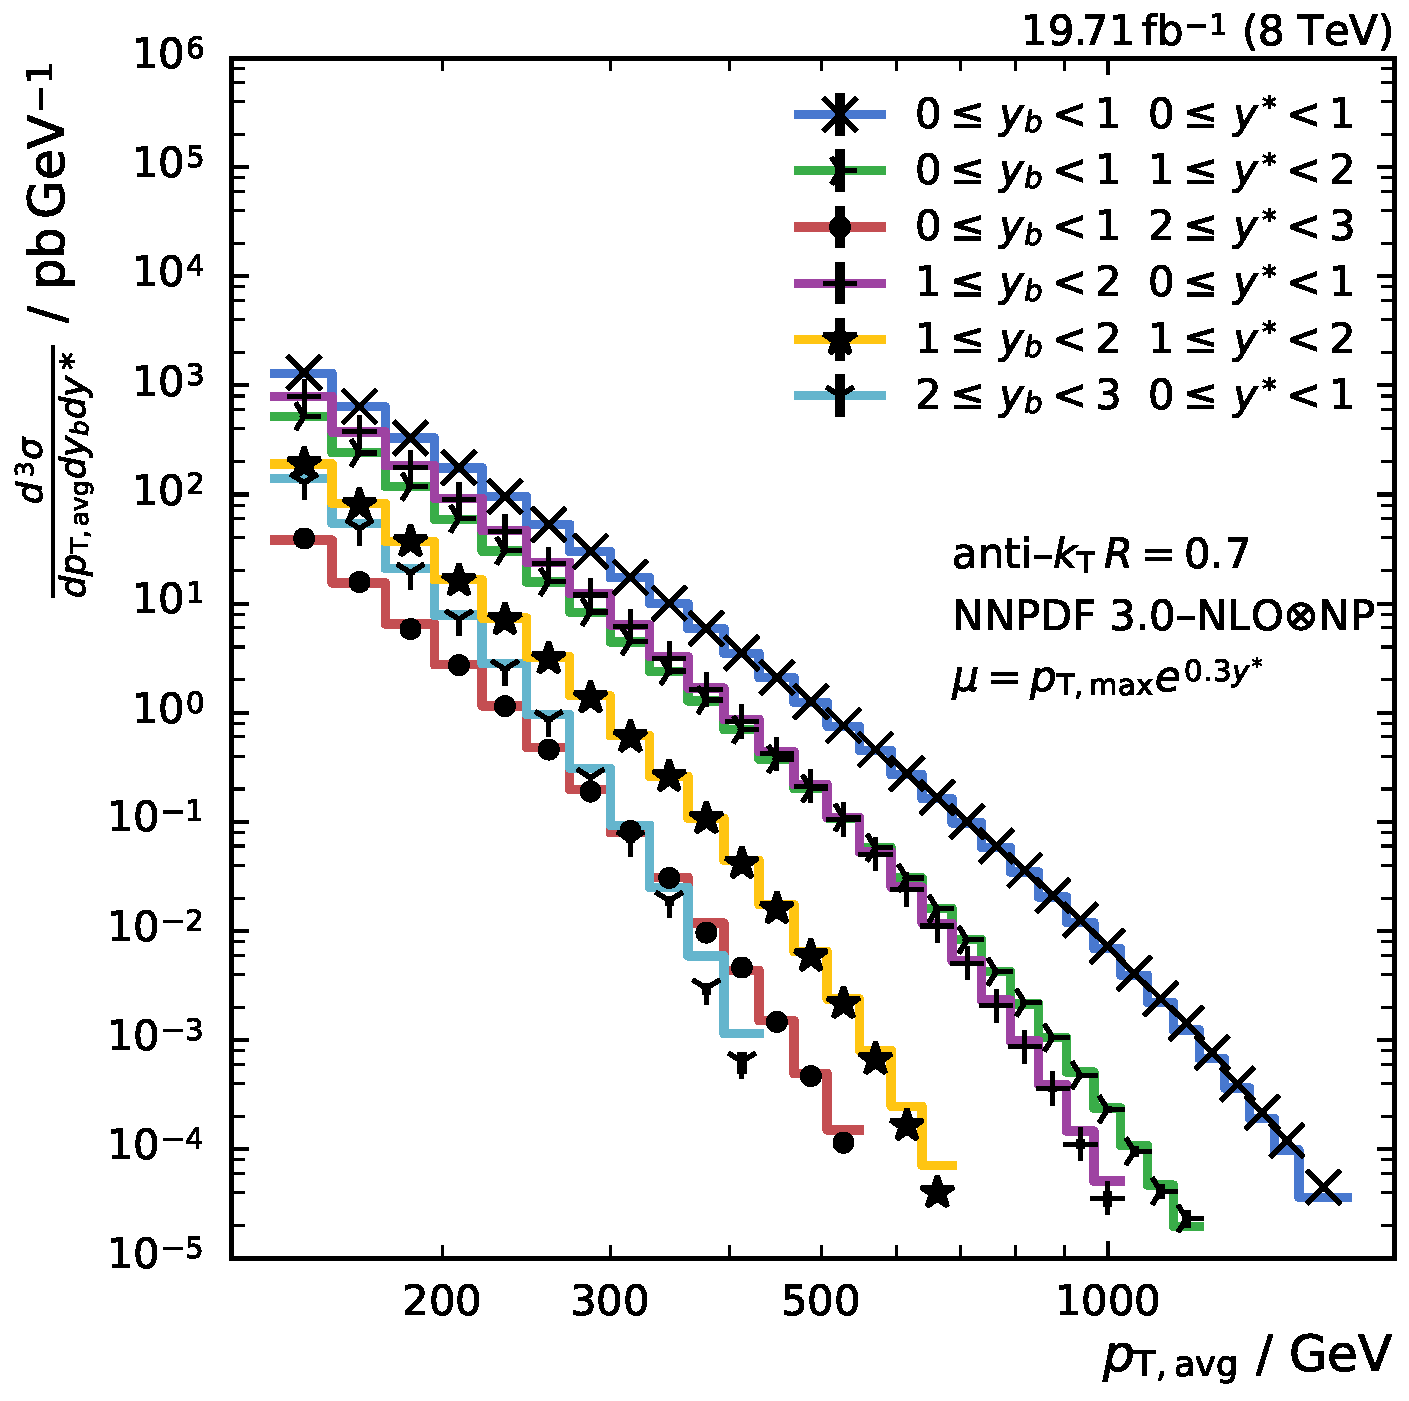
\includegraphics[width=0.45\textwidth]{figures/measurement/ptavg_spectrum.pdf}\hfill
    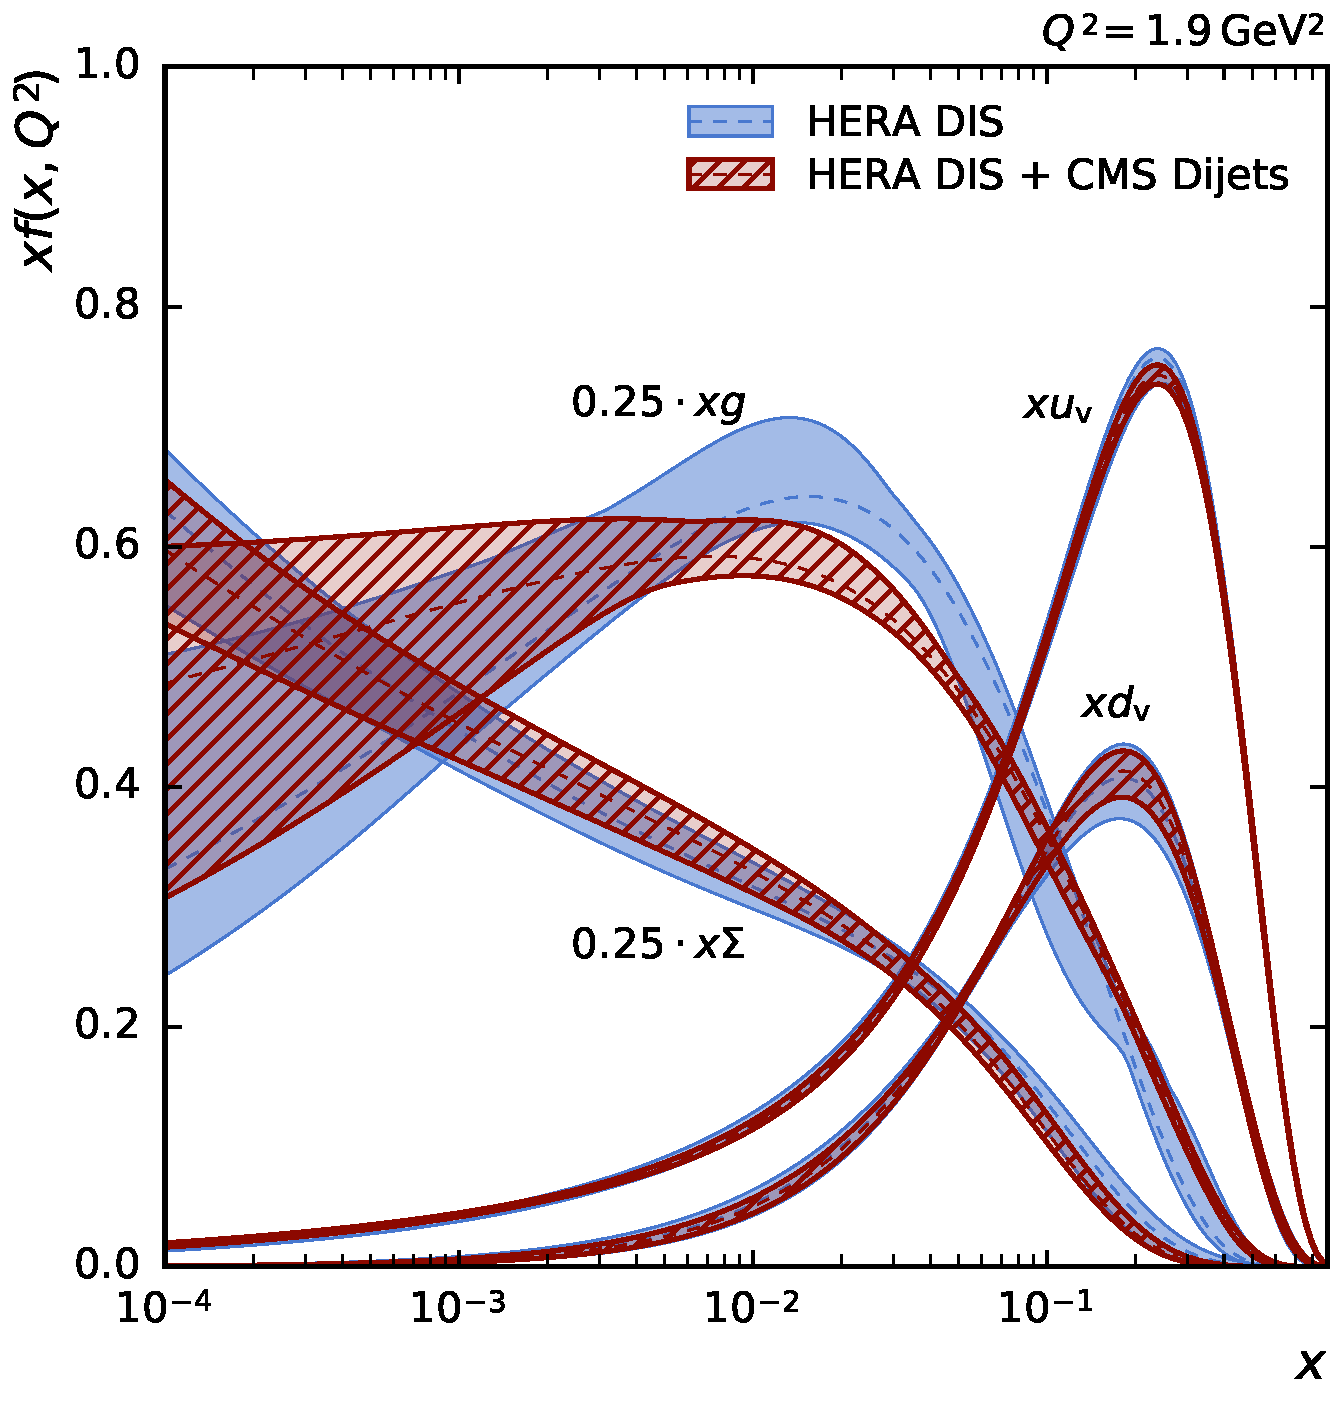
\includegraphics[width=0.45\textwidth]{figures/pdf_constraints/pdfcomp_direct_overview_1.9.pdf}
    \caption[Summary plot of results]{Left:
    The triple-differential dijet cross sections. The data points are indicated by black
    markers, the NLO theory prediction by colored lines. Right: Overview of
    fitted PDFs with and without including the triple-differential dijet
    measurement.}
    \label{fig:conclusion}
\end{figure}

The measurement has been performed using the CMS detector at a center-of-mass
energy of \SI{8}{\TeV} using the complete data set recorded in 2012 comprising
\SI{19.71}{\fbinv}. Thorough studies of trigger efficiencies and jet
identification ensure clean dijet events with a high selection efficiency.
Finally, the measured cross sections have been corrected for detector effects in
an iterative unfolding procedure to be able to compare with theory.

The theoretical predictions were calculated in pQCD at NLO accuracy and were
corrected for non-perturbative effects. Fig.~\ref{fig:conclusion} left shows the
cross sections in the six studied \ystar and \yboost bins. It was found that the
data is well described by the theory over many orders of magnitude. In
phase space regions containing highly boosted dijet events, the data
discriminate between the predictions using different global PDF sets because of
the high experimental precision.

As a consequence, constraints on the PDFs can be provided. The sensitivity of
the PDFs is demonstrated by performing a PDF fit to DIS cross sections of the
HERA experiments and the dijet cross sections measured in this thesis. It was
found that the PDFs are improved when the dijet data are included and the
uncertainties of the PDFs, especially those of the gluon PDF, can be
significantly reduced. Fig.~\ref{fig:conclusion} right demonstrates the PDF
constraints.

The strong coupling constant \asmz was determined by performing a simultaneous
fit of the PDFs and the strong coupling. The extracted value reads as

\begin{equation*}
  \asmz = 0.1188_{-0.0015}^{+0.0015}(\mathrm{exp})_{-0.0002}^{+0.0004}(\mathrm{mod})_{-0.0005}^{+0.0003}(\mathrm{par})_{-0.0010}^{+0.0029}(\mathrm{scale})
\end{equation*}

which is in good agreement with the world average value of the PDG. 

The
uncertainties on \asmz are dominated by the scale uncertainties which will
improve with the availability of NNLO calculations.

The pioneering studies presented in this thesis prove that the triple-differential
measurement of dijet cross sections using the chosen observables are an optimal
approach to perform QCD precision studies with dijets. The uncertainties on the
obtained value of \asmz are dominated by scale unceratinties. In view of
the upcoming NNLO dijet calculations, they should be revisited. The recent
restart of the LHC at $\sqrt{s}=\SI{13}{\TeV}$ opens up a larger accessible
phase space. As soon as enough data has been collected by CMS, further studies
will be possible.

\todo{Concluding sentence}
